\subsection{SqlClient}
Die \eigenName{SqlClient} Klasse verwaltet die Verbindung zum \ac{sql} Server. \\Auf dem \ac{sql} Server sind alle Daten gespeichert, die persistiert werden müssen. 
Die Datenstruktur des Servers ist in Abschnitt \ref{subsec:dataBackend} beschrieben und in \refFig{img:erd} dargestellt.
Diese Struktur ist auf dem \ac{sql} Server vorhanden und wird durch das Script in \refList{list:createSqlTables} konstruiert.
Die \eigenName{SqlClient} Klasse kann ein \ac{sql} Skript ausführen, indem sie es in einzelne Querys zerteilt und diese dann einzeln an den Server sendet.
Das zerteilen eines Skript und das vorbereiten zur Ausführung, ist in der Methode \eigenName{prepareScript} implementiert. 
Beim testen der Methode hat sich herausgestellt, dass diese Funktionalität der \eigenName{sql} Client Klasse Skripte auszuführen, schwieriger zu implementieren ist als anfangs vermutet.
Dies liegt daran, dass das Definieren von \emph{stored Procedures} (siehe Abschnitt \ref{subsec:storedProc}) es nötigt macht den 
%kurze Erwähnung sinn der klasse
%datenaustausch zwischen SqlClient zu abgeleitetrer...(dispatcher.... ) (I/O)
\begin{figure}[ht]
  \centering
  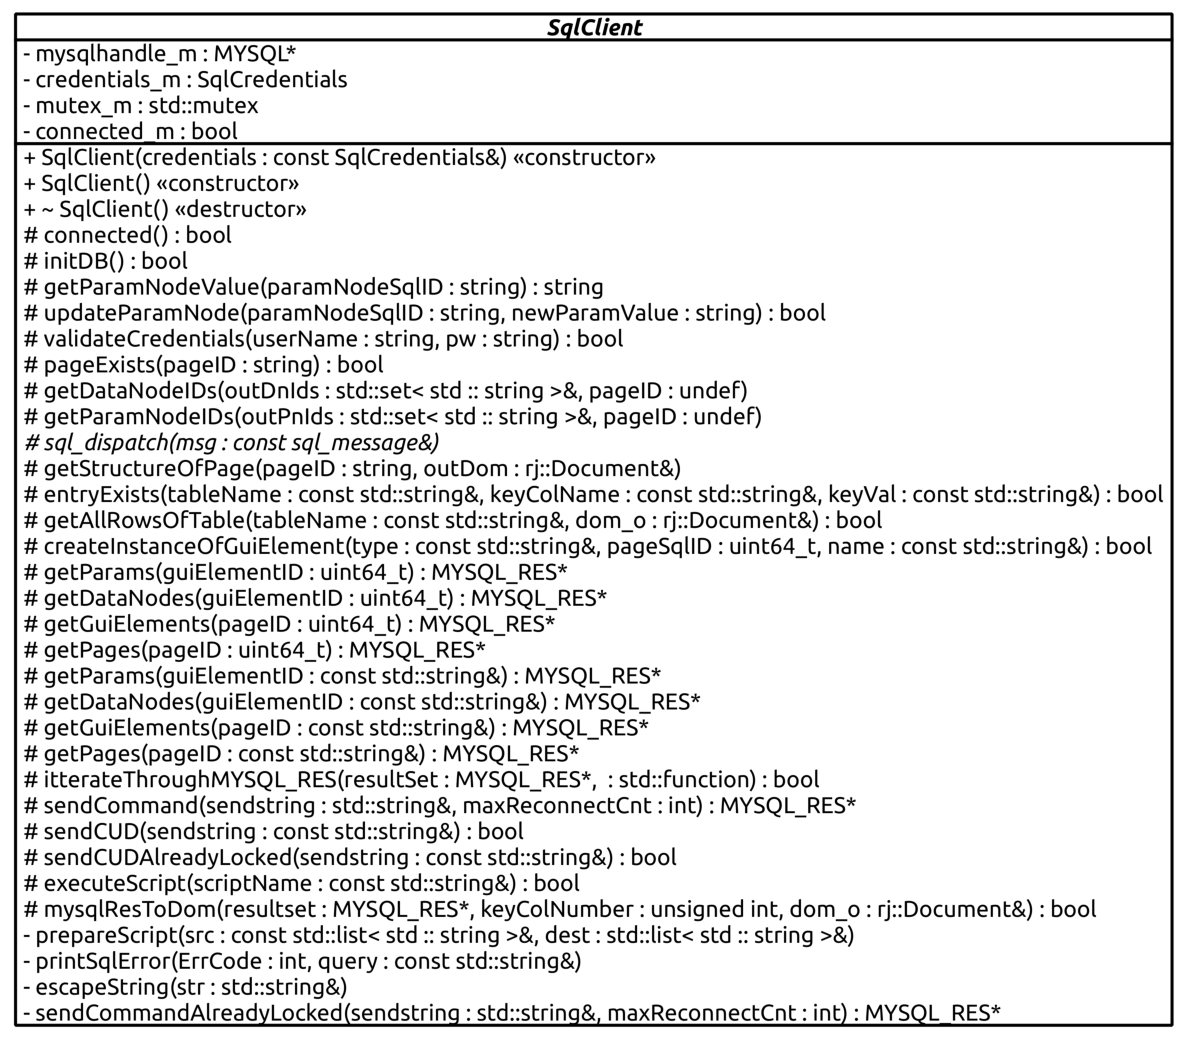
\includegraphics[width=\textwidth]{content/hauptteil/umsetzungPoC/backend/uml/classesOfOverview/SqlClient.pdf}
  \caption{Klassediagramm der Klasse \eigenName{SqlClient}}
  \label{fig:backend:classDiag:SqlClient}
\end{figure}
%beschreibung msg klasse mit diagram
\begin{figure}[ht]
  \centering
  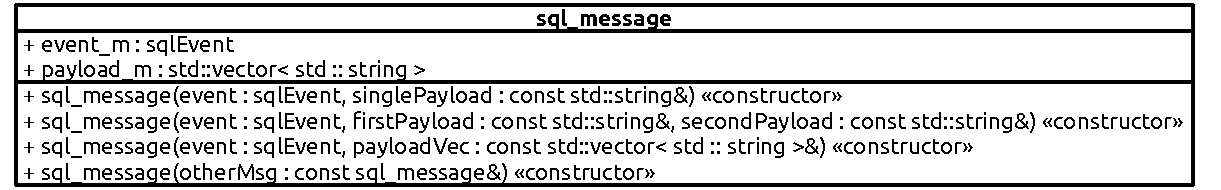
\includegraphics[width=\textwidth]{content/hauptteil/umsetzungPoC/backend/uml/classesOfOverview/sql_message.pdf}
  \caption{Klassediagramm der Klasse \eigenName{sql\_message}}
  \label{fig:backend:classDiag:sqlMsg}
\end{figure}
%dispatcher codeausschnitt
%beschreibung dispatcher